\clearpage
\subsection{Implementation view}
\copied{The development view illustrates a system from a programmer's perspective and is concerned with software management. This view is also known as the implementation view. It uses the UML Component diagram to describe system components. UML Diagrams used to represent the development view include the Package diagram.}
{from wikipedia\\\url{https://en.wikipedia.org/wiki/4\%2B1_architectural_view_model}}

This view deals with, for example, code organization Configuration, building operating system, data base, and middle ware.


\subsubsection{Packages}
The software of the system is divided into several packages. These packages and their relations can be seen in figure~\ref{fig:package-diagram}. 
In this diagram, «use» depicts the use of an interface exposed by a software package, «access» depicts a private import of (parts of) another package, while «import» means a public import of (parts of) another package. 

The diagram contains software packages of the system itself, as well as software packages provided by third parties. The software packages provided by third parties are drawn outside of the `Smart Flood Monitoring System'-box.

\begin{figure}[hb!]
%\centering
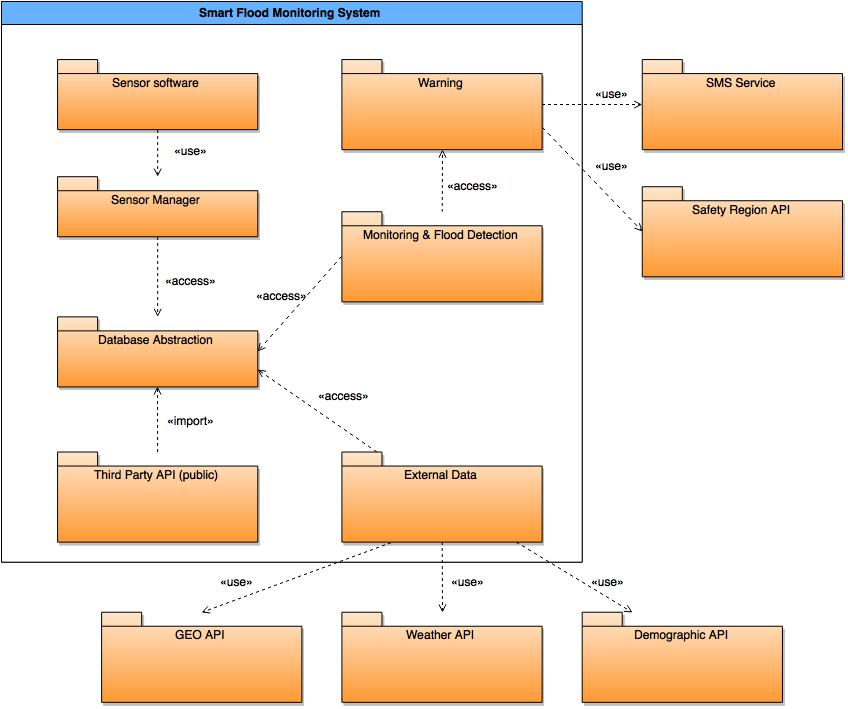
\includegraphics[keepaspectratio=true,width=1.0\textwidth]{{\viewimages/packages}.png}
\caption{Package diagram}
\label{fig:package-diagram}
\end{figure}
